

\documentclass{beamer}


\usetheme{Madrid}

\usepackage[linesnumbered,ruled,vlined]{algorithm2e}
\usepackage{subcaption}
\usepackage{multirow}
\usepackage{booktabs}
\usepackage{threeparttable}
\usepackage{pbox}
\usepackage{ragged2e}
%\usepackage{subfig}
\usepackage{graphicx}
\usepackage{color}
\usepackage{float}
%\usepackage{algorithmic, algorithm2e, float}
\usepackage[absolute,overlay]{textpos}
\usepackage{pbox}
\usepackage{listings}
\usepackage{amsmath}
\usepackage{adjustbox}
\SetAlFnt{\small}
\SetAlCapFnt{\small}
\SetAlCapNameFnt{\small}
\setbeamertemplate{caption}[numbered]

\title[Open Seminar]{Autonomous Vehicles}


\subtitle{and Environment Perception}

\author[A.P. Chouhan]{\textbf{Aaditya~Prakash~Chouhan}}
% - Give the names in the same order as the appear in the paper.
% - Use the \inst{?} command only if the authors have different
%   affiliation.

\institute[] % (optional, but mostly needed)
{
\\	
\textbf{Hackathon Presentation}\\~\\
\textit{aadityaprakash.chouhan@gmail.com}

}
% - Use the \inst command only if there are several affiliations.
% - Keep it simple, no one is interested in your street address.

\date[November 28, 2020]{November 28, 2020}
% - Either use conference name or its abbreviation.
% - Not really informative to the audience, more for people (including
%   yourself) who are reading the slides online

% \subject{Uppaal verification of AIM}
% This is only inserted into the PDF information catalog. Can be left
% out. 

% If you have a file called "university-logo-filename.xxx", where xxx
% is a graphic format that can be processed by latex or pdflatex,
% resp., then you can add a logo as follows:

% \pgfdeclareimage[height=0.5cm]{university-logo}{university-logo-filename}
% \logo{\pgfuseimage{university-logo}}

% Delete this, if you do not want the table of contents to pop up at
% the beginning of each subsection:

% Un-comment these lines to show section layout after every subsection
% \AtBeginSubsection[]
% {
%   \begin{frame}<beamer>{Outline}
%     \tableofcontents[currentsection,currentsubsection]
%   \end{frame}
% }

% Let's get started
\begin{document}

\begin{frame}
  \titlepage
\end{frame}

\begin{frame}{Outline}
  \tableofcontents
  % You might wish to add the option [pausesections]
\end{frame}

% Section and subsections will appear in the presentation overview
% and table of contents.

\section{Autonomous Vehicle}
\begin{frame}{Autonomous Vehicle}
	An Autonomous Vehicle (AV) has an autonomous driver agent for the lateral and/or longitudinal control of the vehicle in some or all driving modes and conditions.\\~\\
	An AV makes use of various sensors for perception of the environment and localization. Lidar, Radar, Sonar, Camera, GPS, IMU (Inertial Measurement Unit), etc. are examples of AV sensors.
	\begin{figure}
		\centering
		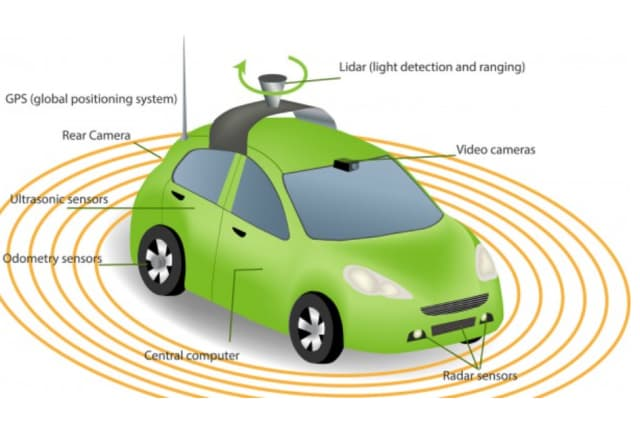
\includegraphics[scale = 0.25]{figures/AV sensors image coutsey_engineering}
		\caption{Sensors used in an AV}
		\label{avsensors}
	\end{figure}
\end{frame}
\begin{frame}{Autonomy Levels of AV}
	The level of autonomy an AV possess depends on:
	\begin{itemize} 
		\item Autonomous control over lateral and/or longitudinal movement,
		\item Who performs the object and event detection and response functionality
		\item The operational design domain of the vehicle\\~\\
		\end{itemize}
	Based on the above mentioned factors, 6 levels of autonomy are defined by the Socitey of Automotive Engineers (SAE) \footnotemark
	\footnotetext{SAE J3016: \textit{Levels of Driving Automation}}
\end{frame}

\begin{frame}{SAE Autonomy Levels}
	\begin{figure}
		\centering
		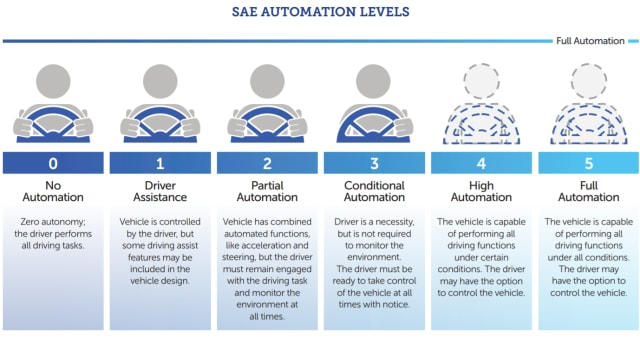
\includegraphics[width = \textwidth]{figures/SAE levels image coutsey_SAE}
		\caption{SAE autonomy levels (\textit{image courtesy of SAE})}
		\label{saelevels}
	\end{figure}
\end{frame}

\begin{frame}{AV Classification}
Autonomous vehicles are classified on the basis of functionalities performed by the autonomous driving system and the driver present in it.\\
Let us first discuss some key components of AV and some associated terms.

\begin{itemize}
    \item \textbf{Driving Task}: It is a broad terms that includes most of the operations required for autonomous driving. It includes
    \begin{itemize}
        \item Environment Perception
        \item Motion Planning
        \item Motion Control
    \end{itemize}
    \item \textbf{Object and Event Detection and Response}: It refers to detection of object and events around the vehicle and reacting to them in appropriate way.
    
    \item \textbf{Operation Design Domain}: This defines the environment in which the AV is set or designed to operate.
    
\end{itemize}
    These three factors mentioned above decide the level of autonomy possessed by the AV.
\end{frame}

\begin{frame}{AV Hardware Architecture}
    \textbf{Perception Hardware}:\\
    This class of hardware gains knowledge of the environment and every object in it. This is required to detect drivable surface and obstacles. These obstacles can be either static or dynamic. Examples of static obstacles are: 
    \begin{itemize}
        \item Road and lane markings
        \item Traffic lights
        \item Traffic signs
        \item Road curbs
        \item Construction signs, obstructions, etc.
    \end{itemize}
    Dynamic objects include:
    \begin{itemize}
        \item Other vehicles
        \item Pedestrians
        \item Animals
    \end{itemize}
\end{frame}

\begin{frame}{Perception Hardware}
    The hardware generally required for environment perception include:
    \begin{itemize}
        \item Camera: A passive sensor i.e. requires external light. Key comparison matrix are field of view, resolution and dynamic range.
        \item LIDAR: An active sensor. Practically unaffected by lighting conditions. Key comparison matrix are resolution and range.
        \item RADAR: They come in short range and long range. Radars are very robust against weather conditions and precipitation. Key performance matrix are field of view and position and velocity accuracy.
        \item SONAR: Work on sound waves rather than radio waves as in the case of RADAR. They are very useful for short range obstacle detection such as while parking.
    \end{itemize}
\end{frame}

\begin{frame}{AV Hardware}
    Other than perception hardware, which are all \textit{exteroceptive} sensors, other class of sensors are also present in AV which are required for detecting ego parameters such as position, velocity, orientation. These are known as \textit{proprioceptive} sensors and include:
    \begin{itemize}
        \item Global Positioning System
        \item Wheel odometers
        \item Inertial Measurement Unit device\\~\\
    \end{itemize}
    An AV also requires hardware for computational purposes. Graphical Processing Units (GPU), Field Programming Gate Array (FPGA), Application Specific Integrated Circuits (ASIC) are examples of such hardwares.
\end{frame}

\begin{frame}{AV Software Architecture}
    The hardware components discussed above pass on a raw data in the form of numbers.  For instance, an image returned from a camera is actually a two-dimensional array of pixel values and each pixel value is an array of three values corresponding to the intensities of the three channels present in a colored image.\\
    
     A possible software architecture of an autonomous vehicle has the following decomposition into the following five parts:
     \begin{itemize}
         \item Environment perception
         \item Environment mapping
         \item Motion planning
         \item Vehicle controller
         \item System supervisor
     \end{itemize}
\end{frame}


\section{Environment Perception}

\begin{frame}
	\tableofcontents[currentsection,currentsubsection]
\end{frame}
%\subsubsection{Autonomous Vehicles}
\begin{frame}{Environment Perception}
The objective of environment perception in autonomous vehicles is to detect all the moving and static objects around vehicle that can have influence on its driving operation. It includes
\begin{itemize}
    \item Lane detection
    \item Traffic sign detection
    \item Pedestrian, cyclists, other vehicle detection and tracking.
\end{itemize}
These detection are made using various perception sensors discussed previously.

\end{frame}

\begin{frame}{Environment Perception}
    Perception sensors detect objects present around vehicles. The output of these sensors are in the form of numerical values that has to be filtered or transformed and then interpreted to gain information.\\~\\
    For instance, camera captures are generally processed before using them for detection purpose. This include camera calibration, perspective transformation, color channel transformation etc. 
    
\end{frame}
\begin{frame}{Environment Perception}
    The processed data from perception sensors are then used by Networks of detection networks which are generally deep neural networks pre-trained using real-world data.\\~\\
    Such machine learning and deep learning based detections are used for classification operations such as pedestrian, cyclists detection, semantic segmentation, traffic sign classification, driveable road detection.
\end{frame}

%\begin{frame}{Intelligent Transportation System}
%	The following figure shows a generalized architecture for an ITS.
%	
%\end{frame}




\begin{frame}
	\begin{center}
		\Huge Thank You!
	\end{center}
\end{frame}



\end{document}

